\documentclass{article}
\usepackage[english]{babel} 
\usepackage{multicol}
\usepackage{graphicx}
\usepackage{hyperref}
\hypersetup{
    colorlinks=true,
    urlcolor=green,
}
\usepackage{hypcap}
\usepackage{makecell}
\usepackage[a4paper, margin=1in]{geometry}
\usepackage{float}
\usepackage{listings}
\usepackage{xcolor}
\usepackage{caption}


% Define PseudoCode language
\lstdefinelanguage{PseudoCode}{
	morekeywords={class, method, end, for, if, else, then, emit, clear, flush, context, value, retrieve_file_name, initialize, cleanup},
	sensitive=true,
	morecomment=[l]{//},
	morestring=[b]"
}

% Set default style for listings
\lstset{
	language=PseudoCode,
	basicstyle=\ttfamily\small,
	keywordstyle=\color{blue}\bfseries,
	commentstyle=\color{gray},
	stringstyle=\color{teal},
	numbers=left,
	numberstyle=\tiny\color{gray},
	stepnumber=1,
	numbersep=5pt,
	breaklines=true,
	frame=single,
	tabsize=2,
	showstringspaces=false
}



\title{Cloud Computing - Project Report \\ Cloud-Busters}
\author{
    Hajar Makhlouf  \\ h.makhlouf@studenti.unipi.it \and 
    Lorenzo Vezzani \\ l.vezzani1@studenti.unipi.it \and
    Francesco Panattoni \\ f.panattoni2@studenti.unipi.it}

\begin{document}
	
	\maketitle
	
	\begin{center}
		\scriptsize
		\href{https://github.com/lorenzo-vezzani/inverted-index-and-search}{https://github.com/lorenzo-vezzani/inverted-index-and-search}
	\end{center}

	
	\pagenumbering{arabic}
	
	\begin{multicols}{2}
	\section{Introduction}
Our project for the Cloud Computing course involves developing a basic search engine backend through the construction of an \textbf{Inverted Index}, a fundamental data structure in information retrieval systems such as \textbf{Google Search}. The main goal is to process a collection of text files and efficiently map each word to the files in which it appears, along with the frequency of its occurrences. Subsequently we had to analyze and compare the performance of a Java-based application using the \textbf{Hadoop} framework with that of a Python-based application using the \textbf{Spark} framework. Finally we have to build a \textbf{search query} in Python based on the inverted indexes produced. 

We tried to make the code as optimized as possible by doing a lot of tests to try to optimize the execution time and memory usage.



	\section{Equipment}
The tests were conducted on three identical virtual machines, each configured with the following hardware and software specifications:
\begin{itemize}
	\item \textbf{CPU}: 2 virtual CPUs (vCPUs), mapped to Intel(R) Xeon(R) Silver 4208 CPU @2.10GHz, provided via KVM virtualization
	\item \textbf{RAM}: 6.8 GB of system memory
	\item \textbf{Disk}: 39 GB of allocated virtual storage (ext4 filesystem)
	\item \textbf{Operating System}: Ubuntu 22.04.1 LTS (Jammy Jellyfish), 64-bit
\end{itemize}
	\section{Dataset}
We selected a 1583.5 MB corpus of 2,685 plaintext files from \href{Project Gutenberg}{https://www.gutenberg.org/}, , covering diverse fields including philosophy, science, theology, psychology, literature and other cultural subjects, to stress and tests our indexer across a broad range of real-world texts. This variety tests the system against typical literary content as well as challenging patterns, mirroring real-world search engine demands on both natural language and specialized data. File sizes vary from 5 KB to 250 MB: most are under 1 MB (reflecting typical book chapters or short essays), 329 fall between 1 MB and 7 MB (full-length books) and one extreme outlier ("Human\_Genome\_Project-Chromosome\_1.txt", 250 MB) contains raw nucleotide sequences. Including this genomic text deliberately exposes our inverted-index builder to vast, mostly unique tokens—mimicking workloads with high vocabulary cardinality and ensuring our system handles both common-word skew and near-unique string distributions. By including files ranging from kilobytes to megabytes, the dataset enables a rigorous evaluation of how indexing and search-query systems scale with input size. 



	\section{MapReduce and Hadoop code}
The system uses MapReduce, via the Hadoop framework, to process large-scale data efficiently. The Hadoop cluster is optimized for virtual machines with limited memory through customized YARN and MapReduce settings. YARN manages resources and memory (up to 5 GB per node), while MapReduce configurations allocate 2048 MB to key tasks, with JVM heaps limited ot 1536 MB. 

...


	\section{Spark code}
The Spark-related Python code was implemented based on the functional patterns and structure demonstrated during the lectures. \textbf{Apache Spark} is an open-source, distributed data processing engine designed for fast in-memory analytics and large-scale workload orchestration. Spark doesn’t strictly use \textbf{MapReduce}, but it supports map and reduce operations but runs them within a more flexible \textbf{DAG} execution model rather than the rigid two-stage MapReduce paradigm.

\vspace{4mm}

Spark jobs were executed on YARN with event logging and the Spark History Server enabled. The configuration included Kryo serialization, dynamic allocation with 3 executors (2 cores and 3GB RAM each), and speculative execution to handle stragglers—ensuring effective resource utilization and monitoring.

\vspace{4mm}

\textbf{RDD\_inverted\_index\_search.py} constructs an inverted index using \texttt{RDDs}. It loads documents from HDFS via \texttt{wholeTextFiles}, generating \texttt{(path, content)} pairs. Text is tokenized by lowercasing, removing non-alphanumerics, and splitting into words, producing key-value pairs of the form: $ ((\textbf{word}, \textbf{docID}), 1) $

These are aggregated using \texttt{reduceByKey}, mapped to \texttt{(word, (docID, count))}, and grouped by key to produce sorted postings lists. Partitioning is adjusted dynamically (1 partition per 44MB) to ensure workload balance. The final output can be saved as tab-delimited text, JSON, or Parquet, generating a distributed inverted index. This is the format of the final output:

\[
\texttt{word \textbackslash t f.name1:count1 \textbackslash t f.name2:count2}
\]

However, this code exhibited suboptimal performance, which was below our expectations for Spark. Therefore, we developed a second version implemented using Spark \texttt{DataFrames}. Spark's \textbf{DataFrames} wrap RDDs with a schema and declarative API, letting Spark Catalyst optimizer and Tungsten execution engine apply column-level and query-plan optimizations for far better performance and memory use than raw RDDs. 

In the new \textbf{inverted\_index\_search.py}, it first loads each specified path into a unified DataFrame annotated with a filename column, gracefully skipping any unreadable files. It then applies a sequence of Spark SQL transformations: all non‐alphanumeric characters are stripped via \texttt{regexp\_replace}, text is lowercased and split on whitespace and each word is exploded into its own row. Empty tokens are filtered out to ensure data quality. So we have a more optimized \textbf{tokenization}. In the next phase, the code groups by word and filename to compute per‐document term frequencies, then concatenates these as filename:count strings. A second grouping by word collects and sorts the full postings list into an array, producing one row per unique term with its complete, ordered document list. Finally the output is either written as plain text (with words and tab‐separated postings) JSON, or Parquet. This approach leverages Spark’s built‐in DataFrame optimizations and avoids manual RDD manipulations while delivering a scalable inverted index. 




	\section{Non‑parallel code}
The non‑parallel Python implementation builds an inverted index on a single node using a SPIMI (Single Pass In‑Memory Indexing) approach. It parses command‑line arguments for local or HDFS input/output URIs, optional size limits, and verbosity via \texttt{argparse}. Text files are read (either from HDFS via \texttt{hdfs.InsecureClient} or from the local filesystem), normalized (punctuation and underscores replaced by spaces), tokenized, and accumulated in an in‑memory index. Every \texttt{BLOCK\_SIZE} files—or when the size limit is reached—the current postings are flushed to a sorted block file in a temporary directory.  
After all blocks are written, a multi‑way merge using a min‑heap combines block files into a single output (written back to local or HDFS), preserving term order and aggregating postings. The script prints a concise summary of block construction time, merge time, total runtime, and memory usage.  

	\section{Search Query System}
The accompanying \texttt{search\_query.py} script is compatible with inverted indexes produced by all implementations. It uses \texttt{build\_term\_offset\_index} to create an in-memory mapping of terms to file offsets, enabling random-access reads during search and minimizing I/O. The \texttt{search\_optimized} function processes user queries by normalizing terms and retrieving relevant postings. It computes the intersection of filenames across query terms and returns a sorted list, omitting term frequencies in accordance with project requirements. The interface supports continuous querying and exits cleanly on \texttt{Ctrl+D}.

Although not scalable like Hadoop or Spark, the non-parallel solution offers a lightweight, easy-to-analyze benchmark for small datasets, helping assess the overhead introduced by distributed frameworks. Its performance metrics are evaluated alongside the parallel implementations in the following section.
	\section{Tests and Results}

\subsection{A first comparison}
For the performance evaluation, four versions of the MapReduce implementation were considered: 
\texttt{Hadoop-noimc}\footnote{IMC stands for \textit{in-mapper combining}}, 
\texttt{Hadoop-imc}, \texttt{Spark-Dataframe} and \texttt{Spark-RDD}. Three metrics were used: \textbf{Execution time}, \textbf{Aggregate resource allocation}\footnote{Aggregate resource allocation shows the total amount of primary memory occupied by the application over time [MB$\cdot$s].} and \textbf{Shuffle bytes}. The comparison was conducted using datasets of: 
\texttt{128MB}, \texttt{256MB}, \texttt{512MB}, \texttt{1024MB}, and \texttt{1583MB}.\\
From the execution time histograms (Fig.~4) it's clear that Hadoop-noimc combiner performs poorly on both small and large datasets. Spark-RDD, instead, turns out to have comparable results to Hadoop-imc combining and Spark-dataframe for small datasets. However, when increasing the dataset, it becomes even worse than Hadoop-noimc. The execution time of Hadoop-imc and Spark-Dataframe is comparable for each input size. \textbf{Non-Parallel Execution}, on the other hand, consistently shows the worst performance as dataset size grows, clearly highlighting the benefits of distributed computing for large-scale data processing.\\
The aggregate resource allocation graph (Fig.~5) closely resembles the execution time graph. This is because aggregate memory usage is strongly correlated with execution time. However, it is also evident that, for the same execution time, Spark programs use more memory than Hadoop ones. This confirms that Spark relies more heavily on in-memory processing, whereas Hadoop performs more disk-based I/O operations. Dividing average aggregate resource allocation by average execution-time, we can obtain average resource allocation. From the following table, relative to the 1583MB case, it is also clearer that the Spark versions exploit more RAM than the Hadoop ones.
\begin{table}[H]
	\centering
	\begin{tabular}{lc}
		\hline
		\textbf{Version} & \textbf{Avg. Memory (MB)} \\
		\hline
		NO-IMC    & 9785.71 \\
		IMC  & 10297.36 \\
		DataFrame & 11008.17 \\
		RDD       & 12745.41 \\
		\hline
	\end{tabular}
	\label{tab:avg-mem}
\end{table}
The last histograms (Fig.~6) are dedicated to shuffle bytes: the amount of MB received by reducers. For small datasets the result is pretty much the same for every version of the application. Starting from 512 MB the shuffle bytes of the RDD version increase significantly until they are extremely more in the version with 1583MB. This is due to the fact that a lot of \textbf{wide transformation} are used, such as: \texttt{repartition} (used to load balancing data), \texttt{groupByKey}, \texttt{reduceByKey} and \texttt{sortyByKey}.\\
Indeed, the CPU time\footnote{CPU time is the total time the CPU actually executed instructions from a process, summed across all cores used.}, relative to the 1583MB case, as shown in the following table, is very low in the RDD-version, due to high number of I/O operations resulting from wide transformations. It is also evident that the CPU time is very high in Hadoop-noimc, the main reason behind this is the high amount of \texttt{emit()} called in the map phase.
\begin{table}[H]
	\centering
	\begin{tabular}{lc}
		\hline
		\textbf{Version} & \textbf{CPU Time (s)} \\
		\hline
		NO-IMC    & 1154.49 \\
		IMC  & 642.85 \\
		DataFrame & 521.85 \\
		RDD       & 82.59 \\
		\hline
	\end{tabular}
	\label{tab:avg-cpu-time}
\end{table}
\begin{figure}[H]
	\centering
	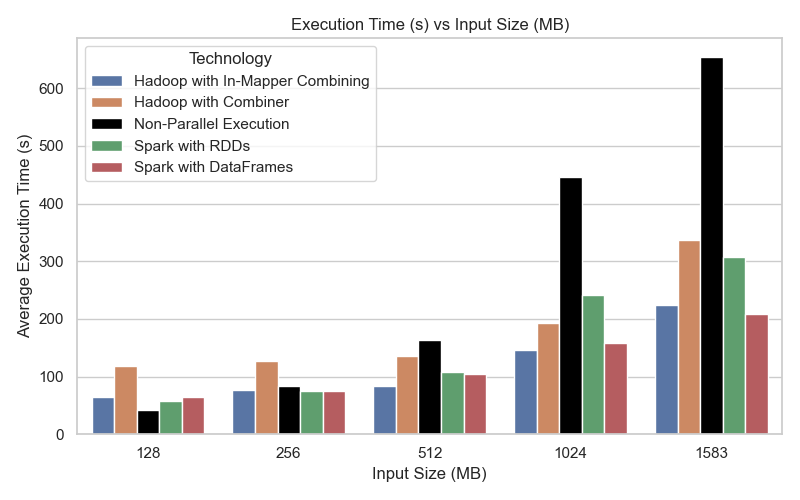
\includegraphics[width=0.444\textwidth]{images/Fig_Execution_Time.png}
	\caption{Execution time plot}
	\label{fig:execution-time}
\end{figure}
\begin{figure}[H]
	\centering
	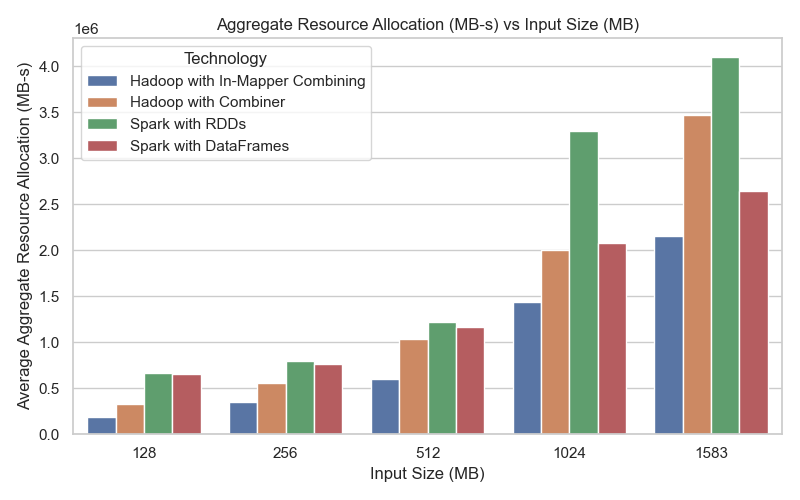
\includegraphics[width=0.444\textwidth]{images/Fig_Aggregate_Resource_Allocation.png}
	\caption{Aggregate resource plot}
	\label{fig:aggregate-resource-allocation}
\end{figure}
\begin{figure}[H]
	\centering
	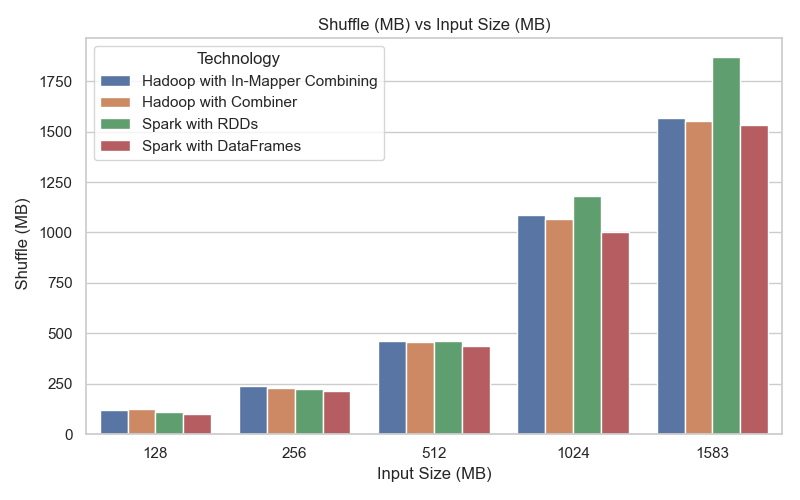
\includegraphics[width=0.444\textwidth]{images/Fig_Shuffle.png}
	\caption{Shuffle plot}
	\label{fig:shuffle}
\end{figure}

\newpage

\subsection{Effect of Reducers on Performance}
The Execution Time image (Fig.~7) shows the impact of varying the number of reducers on the execution time of the Hadoop application. As input size increases, the difference in performance becomes more pronounced. For small datasets (128MB, 256MB and 512MB), the reducer count has minimal impact. However, for larger datasets (1024MB and 1583MB), using more reducers generally leads to lower execution times, with the best performance observed when using 4 reducers. Interestingly, performance slightly degrades when moving from 4 to 8 reducers, likely due to overhead from task coordination and context switching. This suggests that, while increasing reducer count improves parallelism and reduces execution time up to a point, beyond that point the benefits diminish or even reverse. 

For Aggregate Resource Allocation (Fig.~8), despite some small irregularities in the graph, it is easy to see that there is a pattern: it increases as the number of reducers increases. This behavior is expected, as increasing the number of reducers leads to more concurrent tasks executing in parallel, each requiring its own memory space. As a result, the total memory footprint of the application increases with the number of reducers. Although this allows for better task distribution and reduced execution time, it comes at the cost of higher memory consumption. Therefore, there is a trade-off between parallelism and resource utilization, and selecting the optimal number of reducers involves balancing execution efficiency with memory availability.

\begin{figure}[H]
	\centering
	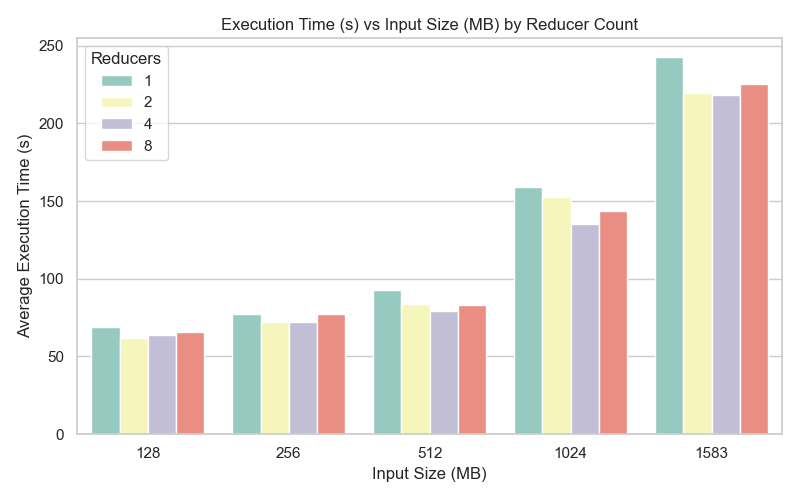
\includegraphics[width=0.5\textwidth]{images/Fig_Reducers_Execution_Time.png}
	\caption{Reducers Execution Time}
	\label{fig:reducer-execution-time}
\end{figure}

\begin{figure}[H]
	\centering
	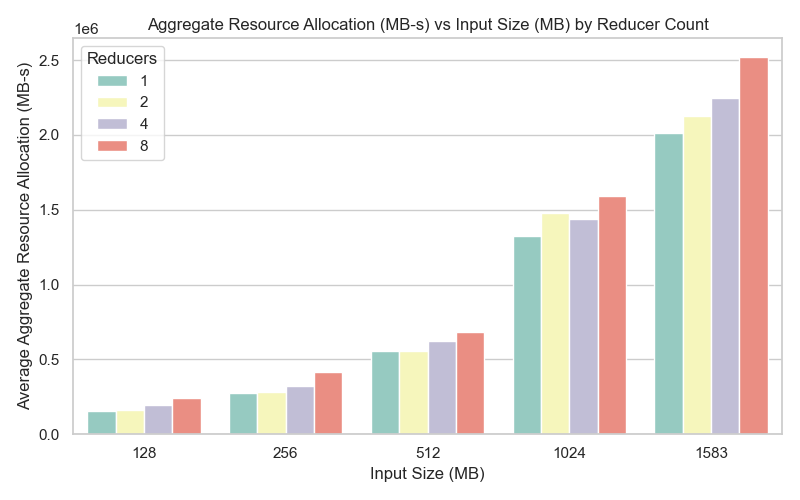
\includegraphics[width=0.5\textwidth]{images/Fig_Reducers_Aggregate_Resource_Allocation.png}
	\caption{Reducers Aggregate Resource Allocation}
	\label{fig:reducer-aggregate-resource-allocation}
\end{figure}

\subsection{Final Considerations}
The comprehensive evaluation across execution time, memory usage and shuffle volume shows that no single implementation universally dominates every metric, but trade‑offs emerge clearly. \texttt{Hadoop-noimc} suffers from both high CPU time (1154.49\,s) and poor scalability, while \texttt{Spark-RDD} achieves the lowest CPU time (82.59\,s) at the expense of excessive shuffle bytes and aggregate resource allocation (12745.41\,MB\,$\cdot$\,s on average). \texttt{Hadoop-imc} improves over \texttt{Hadoop-noimc} by reducing both execution time and memory footprint, yet still lags behind the Spark-based approaches for large datasets.

\texttt{Spark with Dataframes} consistently delivers near‑optimal execution times while keeping both aggregate resource allocation (11008.17\,MB\,$\cdot$\,s) and shuffle volume moderate. This balance of low execution latency, controlled memory consumption and efficient shuffling makes the DataFrame API the best choice for large‑scale word‑count workloads on our cluster. Furthermore, tuning the reducer count to four provides additional speedup in Hadoop jobs, but does not bridge the gap to Spark’s in‑memory processing advantages.

In conclusion, for batch analytics on medium to large datasets, \texttt{Spark with Dataframe} offers the strongest overall performance profile. However, if minimizing memory usage is paramount and data volumes remain moderate, \texttt{Hadoop with In-Mapper Combining} remains a viable alternative.

	\end{multicols}
	
\end{document}